\chapter{Introduction et Fondements Théoriques des Descripteurs Visuels}
\label{chap:intro_descripteurs}

\section{Contexte et Problématique du CBIR}

L'accroissement exponentiel des collections d'images numériques impose le recours à des systèmes d'indexation et d'extraction automatisés. Historiquement, l'accès à ces bases reposait sur la recherche textuelle d'images (\textbf{TBIR} — \textit{Text-Based Image Retrieval}). Néanmoins, le modèle TBIR présente des écueils majeurs : coût prohibitif de l'annotation manuelle, subjectivité perceptive entre annotateurs, ambiguïté polysémique et incapacité à traduire les nuances visuelles fines (textures, gradients, nuances chromatiques).

Pour surmonter ces verrous, la communauté s'est tournée vers la \textbf{recherche d'images par le contenu} (\textbf{CBIR} — \textit{Content-Based Image Retrieval}). Le principe consiste à extraire automatiquement du signal numérique (la matrice de pixels) une signature mathématique compacte appelée \textbf{vecteur de caractéristiques} ou \textbf{descripteur visuel} :
\begin{equation}
    \mathbf{x} = \phi(I) \in \mathbb{R}^d
\end{equation}
La recherche d'images similaires à une requête $I_q$ se ramène alors à une recherche des $k$ plus proches voisins ($k$-NN) au sein de l'espace métrique induit :
\begin{equation}
    \mathcal{S}(I_q, k) = \arg\min_{\substack{\mathcal{C} \subseteq \mathcal{D} \\ |\mathcal{C}| = k}} \sum_{I_i \in \mathcal{C}} \mathcal{D}\big(\phi(I_q), \phi(I_i)\big)
\end{equation}
où $\mathcal{D}(\cdot, \cdot)$ désigne une fonction de distance métrique et $\mathcal{D}$ la base de données globale.

\subsection{Le Fossé Sémantique (\textit{Semantic Gap})}
Le CBIR se heurte au \textbf{fossé sémantique} \cite{smeulders2000} : la disparité intrinsèque entre l'information visuelle brute de bas niveau calculée par l'ordinateur (distributions de couleurs, micro-textures, directions de gradients) et la signification sémantique de haut niveau qu'un être humain associe instantanément à une scène. Pour atténuer ce décalage, un système CBIR doit exploiter des descripteurs complémentaires, des métriques adaptées et des modalités hybrides couplant recherche visuelle et filtrage textuel.

\subsection{Objectifs et Cahier des Charges}
Ce projet d'ingénierie à SUPCOM vise la réalisation d'une plateforme CBIR complète :
\begin{enumerate}[nosep]
    \item Implémentation modulaire de descripteurs de couleur (RGB, HSV), de texture (\textbf{LBP}), de forme (\textbf{HOG}) et de contours (\textbf{MPEG-7}).
    \item Indexation métrique haute performance par \textbf{VP-Tree} pour accélérer la recherche $k$-NN.
    \item Persistance relationnelle \textbf{SQLite} et cache vectoriel binaire optimisé \textbf{NumPy} (\texttt{.npy}).
    \item Moteur de recherche multimodal : filtrage textuel conjonctif, recherche floue (\textit{Fuzzy Search}) et fusion tardive texte-image.
    \item Interface web interactive et moderne sous \textbf{Streamlit} (thème sombre, navigation \textit{Query-by-Example}).
    \item Évaluation quantitative rigoureuse sur le jeu de données de référence \textbf{Caltech-101} ($9~145$ images, $101$ classes).
\end{enumerate}

\section{Espaces Colorimétriques et Histogrammes de Couleur}

La couleur constitue l'indice visuel le plus robuste aux variations d'échelle et aux rotations dans le plan.

\subsection{Espaces RGB et HSV}
L'espace \textbf{RGB} modélise l'image comme un champ additif trichromatique $I_{\text{RGB}}(u, v) = (R, G, B) \in [0, 255]^3$. Malgré sa prévalence matérielle, ses canaux sont fortement corrélés et très sensibles aux variations d'illumination.

L'espace \textbf{HSV} (\textit{Hue, Saturation, Value}) découple la composante achromatique d'intensité lumineuse ($V$) des informations chromatiques pures ($H$, teinte angulaire sur $[0^\circ, 360^\circ]$, et $S$, saturation). Ce découplage assure une grande stabilité face aux ombres et aux variations d'intensité lumineuse pour les pixels saturés ($S > \epsilon$).

\subsection{Formulation de l'Histogramme de Couleur}
Pour une image de $N = W \times H$ pixels discrétisée en $B$ intervalles (\textit{bins}), l'histogramme normalisé par la norme $L_1$ représente la densité de probabilité empirique :
\begin{equation}
    h(k) = \frac{1}{N} \sum_{i=1}^{W} \sum_{j=1}^{H} \mathbf{1}\big( q(I(i, j)) = k \big), \quad k \in \{0, \dots, B - 1\}, \quad \sum_{k=0}^{B-1} h(k) = 1
\end{equation}
Plutôt qu'un histogramme conjoint 3D dont la taille explose de manière cubique ($64^3 = 262~144$ bins), nous adoptons la \textbf{concaténation d'histogrammes marginaux 1D} :
\begin{equation}
    \mathbf{d}_{\text{RGB}} = \big[ \mathbf{h}_R \,\|\, \mathbf{h}_G \,\|\, \mathbf{h}_B \big] \in \mathbb{R}^{3 B_c}
\end{equation}
Avec $B_c = 64$ bins par canal après redimensionnement à $256 \times 256$ pixels, le descripteur présente une dimension compacte $d = 3 \times 64 = \mathbf{192}$, conciliant expressivité et faible coût calculatoire.

\section{Descripteurs de Texture : Local Binary Patterns (LBP)}

Le descripteur LBP \cite{ojala1996, ojala2002} encode l'agencement spatial de la texture locale. Pour un pixel central $(x_c, y_c)$ d'intensité $g_c$ et $P$ voisins $g_p$ disposés régulièrement sur un cercle de rayon $R$ :
\begin{equation}
    \text{LBP}_{P, R}(x_c, y_c) = \sum_{p=0}^{P-1} s(g_p - g_c) \cdot 2^p, \quad s(u) = \begin{cases} 1 & \text{si } u \ge 0 \\ 0 & \text{si } u < 0 \end{cases}
\end{equation}
Les intensités aux coordonnées non entières sont calculées par interpolation bilinéaire.

\begin{figure}[H]
    \centering
    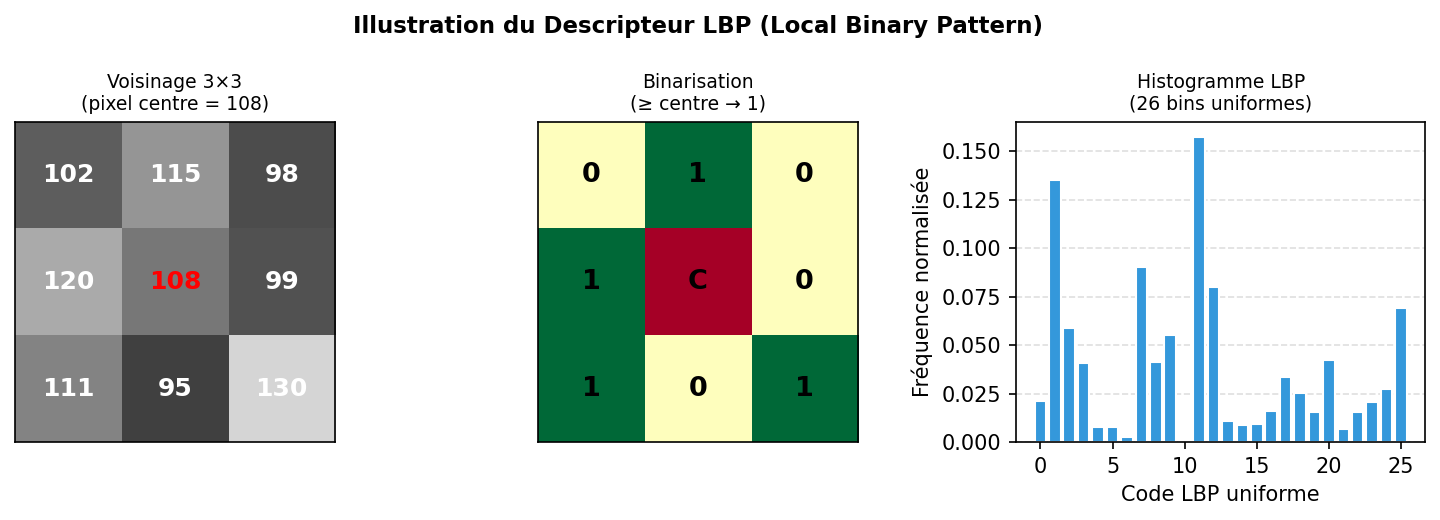
\includegraphics[width=0.88\textwidth]{figures/lbp_illustration.png}
    \caption{Extraction du code LBP : voisinage local, binarisation et histogramme de texture.}
    \label{fig:lbp_schema}
\end{figure}

Un motif est dit \textbf{uniforme} s'il présente au plus deux transitions binaires circulaires ($0 \to 1$ ou $1 \to 0$). Les motifs uniformes capturent les micro-structures essentielles (bords, coins, zones lisses). Avec $P = 24$ et $R = 3$ en mode rotation-invariant uniforme, le vecteur résultant est condensé à seulement \textbf{26 dimensions}.

\section{Descripteurs de Forme : Histogram of Oriented Gradients (HOG)}

Le descripteur HOG \cite{dalal2005} caractérise l'apparence et la silhouette des objets par la distribution des directions des gradients locaux :
\begin{align}
    G_x(x, y) &= I(x + 1, y) - I(x - 1, y), \quad G_y(x, y) = I(x, y + 1) - I(x, y - 1) \\
    m(x, y) &= \sqrt{G_x^2 + G_y^2}, \quad \theta(x, y) = \arctan(G_y / G_x) \bmod 180^\circ
\end{align}
L'image est découpée en cellules de $8 \times 8$ pixels. Pour chaque cellule, les gradients sont accumulés dans un histogramme de 9 orientations non signées par vote bilinéaire. Des blocs couvrants de $2 \times 2$ cellules subissent une normalisation robuste par hystérésis \textbf{L2-Hys} :
\begin{equation}
    \mathbf{v}' = \frac{\mathbf{v}}{\sqrt{\norm{\mathbf{v}}_2^2 + \epsilon^2}}, \quad v''_i = \min(v'_i, 0{,}2), \quad \mathbf{v}_{\text{final}} = \frac{\mathbf{v}''}{\sqrt{\norm{\mathbf{v}''}_2^2 + \epsilon^2}}
\end{equation}
Sur des images normalisées de $128 \times 128$ pixels, la dimension totale est de \textbf{1~764 composantes}.

\section{Le Standard MPEG-7}
Le moteur CBIR intègre également les spécifications des descripteurs MPEG-7 (ISO/IEC 15938) :
\begin{itemize}[nosep]
    \item \textbf{EHD (Edge Histogram Descriptor) :} Distribution spatiale des contours (5 types élémentaires) sur $4 \times 4 = 16$ sous-images ($d = 80$).
    \item \textbf{CLD (Color Layout Descriptor) :} Coefficients DCT 2D basse fréquence de la couleur moyenne sur une grille $8 \times 8$ dans l'espace $YC_bC_r$ ($d = 12$ à $18$).
    \item \textbf{SCD (Scalable Color Descriptor) :} Histogramme HSV projeté par transformée en ondelettes de Haar.
    \item \textbf{CSD (Color Structure Descriptor) :} Accumulation de présence chromatique sous un élément structurant $8 \times 8$.
\end{itemize}

\begin{table}[H]
    \centering
    \small
    \caption{Comparatif des descripteurs visuels implémentés dans la plateforme}
    \label{tab:comparatif_descripteurs}
    \begin{tabular}{lccccc}
        \toprule
        \textbf{Descripteur} & \textbf{Domaine} & \textbf{Dimension} & \textbf{Invariance Rotation} & \textbf{Invariance Échelle} & \textbf{Coût Calcul} \\
        \midrule
        \textbf{RGB Hist.}   & Couleur  & 192   & Totale  & Totale (norm.) & Très faible \\
        \textbf{HSV Hist.}   & Couleur  & 288   & Totale  & Totale (norm.) & Faible \\
        \textbf{LBP Uniform} & Texture  & 26    & Totale  & Modérée        & Très faible \\
        \textbf{HOG}         & Forme    & 1~764 & Faible  & Modérée        & Moyen / Élevé \\
        \textbf{MPEG-7 EHD}  & Contours & 80    & Faible  & Totale (norm.) & Faible \\
        \textbf{MPEG-7 CLD}  & Couleur  & 18    & Nulle   & Totale (DCT)   & Très faible \\
        \bottomrule
    \end{tabular}
\end{table}
